\documentclass[a4paper,11pt]{article}
\usepackage[utf8]{inputenc}


%math
\usepackage{amsmath}
\usepackage{amssymb}
\usepackage{amsfonts}
\usepackage{theorem}
\usepackage{pstricks}
\usepackage{algorithm}
\usepackage{algpseudocode}
\usepackage{enumitem}
\usepackage{ifthen}     % if-then-else command
\usepackage{euscript}
\usepackage{mathrsfs}   %
\usepackage{tabu}
\usepackage{rotating}
\newtheorem{theorem}{Theorem}[section]     %
\newtheorem{definition}{Definition}[section]  %
\newtheorem{proof}{Proof}[section]  %
\newtheorem{lemma}{Lemma}[section]  %
\newtheorem{proposition}{Proposition}[section] %
\newtheorem{remark}{Remark}[section] %
\DeclareMathOperator{\sgn}{sgn} % enable partial derivative
\usepackage[super]{nth} % enable easy first and second etc
\usepackage{comment} % to enable block of comment
\DeclareMathOperator*{\argmax}{arg\,max} %enable argmax
\DeclareMathOperator*{\argmin}{arg\,min} %enable argmin
\newcommand{\innerproduct}[2]{\langle #1, #2 \rangle} %enable innerproduct

\usepackage{pdfpages}

%formatting
\usepackage{hyphenat}
\usepackage{enumerate}  % tm make it possible to define the numbers (A,a, ...)
\usepackage{float}      % you can define 'H' so that floats are forced to be putted 'here'
\usepackage{afterpage}  % adds \afterpage command, which makes it possible to issue \afterpage{\clearpage} which flushes all floats after this page
\usepackage{rotating}
\usepackage{ulem}       % for underlining text \ul{...}
\usepackage{derivative} % for partial deivative

%graphics
\usepackage{epic,eepic}
\usepackage{graphicx}
\usepackage{epstopdf}
\usepackage{caption}
\usepackage{subcaption}
\usepackage{tabularx}
\usepackage{bigstrut}
\usepackage{color, xcolor}

% code
\usepackage[framed,numbered,autolinebreaks,useliterate]{mcode}

%tables
\usepackage{listings}
\usepackage{tabularx}
\usepackage{multirow}   % multirow{nrows}[bigstruts]{width}[fixup]{text} multirow cells
\usepackage{listings}
\usepackage{hhline}     % generates nicer table lines (without missing pixels) + more flexible
\usepackage{colortbl}   % for coloured columns
\usepackage{threeparttable} % adds the possibility to add footnotes in tables
\usepackage{longtable}  %for tables spanning multiple pages

%referencing
\usepackage{cite}
\usepackage{bbm}
\usepackage{url}
\usepackage{hyperref}
\hypersetup{colorlinks=true,
            citecolor=black,
            linkcolor=red,
            citebordercolor=blue,
            urlcolor=magenta,
            linktocpage,
            plainpages=false}
\usepackage{listings}
\usepackage{comment}
\numberwithin{equation}{section} % for the formulas order

%Matlab code
\usepackage{listings}
%\usepackage[framed,numbered,autolinebreaks,useliterate]{mcode}

%----------------------
\PassOptionsToPackage{normalem}{ulem}
\topmargin 0.4cm
\oddsidemargin -0.1cm
\textwidth  15cm
\headheight 0.0cm
\textheight 22.2cm
\parindent  0mm
\parskip    10pt
\tolerance  1000
%----------------------

\title{Technical Report}
\author{Theodors Katzalis}
\date{March 2023}

\begin{document}

\maketitle

\tableofcontents
\newpage

\section{Introduction}
\label{intro}

\subsection{Study Phase} (this subsection can be remove in final report)

Part 1: Line Search methods

\begin{itemize}
\item Chapter 1 and Chapter 2 of ref.1
\item Chapter 3 : Sections 3.1, 3.2, 3.3 and 3.5 of ref.1
\item Zhang, H. and Hager, W.W. (2004) A Nonmonotone Line Search Technique and Its Application to Unconstrained Optimization. SIAM Journal on Optimization, 14, 1043-
1056.
\end{itemize}

Part 2: Quasi-Newton methods
\begin{itemize}
\item Chapter 6 : Sections 6.1 and 6.4 of ref.1
\item Chapter 7 : Section 7.2 of ref.1
\item Chapter 2 : Section 2.2 of ref.2
\end{itemize}

Part 3: L-BFGS-B
\begin{itemize}

\item Byrd, R. H.; Lu, P.; Nocedal, J.; Zhu, C. (1995). A Limited Memory Algorithm for
Bound Constrained Optimization. SIAM J. Sci. Comput. 16 (5): 1190–1208.
doi:10.1137/0916069. S2CID 6398414.

\item Zhu, C.; Byrd, Richard H.; Lu, Peihuang; Nocedal, Jorge (1997). L-BFGS-B: Algorithm 778: L-BFGS-B, FORTRAN routines for large scale bound constrained optimization. ACM Transactions on Mathematical Software. 23 (4): 550–560.

\item Morales, J. L.; Nocedal, J. (2011). Remark on quote;algorithm 778: L-BFGS-B:
Fortran subroutines for large-scale bound constrained optimization; ACM Transactions on Mathematical Software. 38: 1–4.

\end{itemize}

References
\begin{itemize}
 \item Ref. 1: Numerical optimization, J. Nocedal and S. Wright, Second Edition (digital copy of the book can be found \url{https://www.csie.ntu.edu.tw/~r97002/temp/num_optimization.pdf}
\item Ref. 2: Nonlinear programming, D. Bertsekas, Third Edition, Athena Scientfic.
\end{itemize}

Knowledge consolidation of math optimization around Quasi-Newton methods via concept summarizing and exercises solving of \cite{nocedal1999numerical, bertsekas1997nonlinear}.

\subsection{Updates}
\begin{itemize}
    \item \textbf{Week 11-18/04/2023:}
    \begin{itemize}
        \item Add documentation to the functions `newton.m` and `steepest\_descent.m` with examples on how to use it. Otherwise, the jupyter notebook can be used as a reference point on how to call these methods.
        \item Add wolfe strong line search method. For the interpolation step, we use the simple bisection method instead of a more sophisticated solution with cubic or quadratic interpolation.
        \item Add more functions with more than 2 dimensions as provided on mattermost to test the functions.
        \item Add plots when finishing the executing of the line search methods to illustrate the progress of the algorithm.
        \item The jupyter notebook has been updated to include the new functions and to show the plots. (Currently a pdf is exported to include it on this report. When there is access to a git host system, a link will be used to avoid the sync issue).
    \end{itemize}
    \item \textbf{Week 18-27/04/2023:}
    \begin{itemize}
        \item Document how to execute the functions and provide a demo script along with the jupyter notebook (moved to appendix).
        \item Use new starting points.
        \item Draw 3d plots using contour and 3d lines.
        \item Create a table with the results of the analysis.
    \end{itemize}
    \item \textbf{Week 28-04/05/2023:}
    \begin{itemize}
        \item Implement the nonmonotone line search technique of Zhang-Hager.
    \end{itemize}
\end{itemize}

\pagebreak

\section{}

Problems listed on Chapter 2 of ref \cite{nocedal1999numerical}:

\label{rosenbrock}
\subsection{}

\textbf{Problem}

Compute the gradient $\nabla f(x)$ and Hessian $\nabla^2 f(x)$ of the Rosenbrock function.

\begin{equation}
    f(x) = 100(x_2 -x_1^2)^2 + (1-x_1)^2
\end{equation}

Show that $x^{\ast} = (1, 1)^{T}$ is the only local minimizer of this function, and that the Hessian matrix at that point is positive definite.


\textbf{Solution}

\begin{align}
    \nabla f(x) &= (\frac{\partial f}{\partial x_1}, \frac{\partial f}{\partial x_2}) \\
    \nabla f(x) &= (2(200x_1^3 -200x_2x_1 + x_1- 1)), 200(x_2 - x_1^2)) \\
    \nabla^2 f(x) &=
    \begin{bmatrix}
    800x_1^2 - 400(x_2 - x_1^2) +2 & -400x_1 \\
    -400x_1 & 200
    \end{bmatrix}
\end{align}

To find all the possible stationary points and potentially the local minimums we solve $\nabla f(x) =0$ and the only root is $x^{*} = (1,1)$. To check if the stationary point is a local minimum and this case a global minimum, since there aren't any other stationary points, then we have to check if $\nabla^2 f(x^{*})$ is positive definitive and we have:

\begin{equation}
    \nabla^2 f(1,1) =
    \begin{bmatrix}
        802 & -400 \\
        -400 & 200
    \end{bmatrix}
\end{equation}

The eigenvalues for the above matrix are $\lambda_1 \approx 1001.6$ and $\lambda_2 \approx 0.399361$. We can prove that the matrix is positive definite. Thus, the $x^{*} = (1,1)$ is the global minimum of the Rosenbrock function.

\subsection{}

\textbf{Problem}

Show that the function $f(x) = 8x_1 + 12x_2 + x_1^2 - 2x_2^2$ has only one stationary
point, and that it is neither a maximum or minimum, but a saddle point. Sketch the contour
lines of f.

\textbf{Solution}


To find the stationary points we solve $\nabla f(x) = 0$ and we have:
\begin{equation}
    \nabla f(x) = (2(x+4), -4(y-3)
\end{equation}
, thus the only root is $x^{*} = (-4, 3)$. To prove that it is a saddle point, we have to show that some of the eigenvalues of the Hessian matrix are positive and the rest negative. Thus we have:

\begin{equation}
    \nabla^2 f(x) =
    \begin{bmatrix}
        2 & 0 \\
        0 & -4
    \end{bmatrix}
\end{equation}

and eigenvalues $\lambda_1 = -4$ and $\lambda_2 = 2$. The first is positive and the second is negative. Thus, we have proved that the point $(-4, 3)$ is a saddle one.

\begin{figure}[h!]
     \centering
     \begin{subfigure}[b]{0.45\textwidth}
         \centering
         \includegraphics[width=\textwidth]{assets/saddle_3d.png}
         \caption{3D}
     \end{subfigure}
     \hfill
     \begin{subfigure}[b]{0.45\textwidth}
         \centering
         \includegraphics[width=\textwidth]{assets/saddle_contour.png}
         \caption{Contour lines}
     \end{subfigure}
    \caption{}
\end{figure}

\subsection{}

\textbf{Problem}

Let a be a given n-vector, and A be a given n × n symmetric matrix. Compute the
gradient and Hessian of $f_1(x) = a^T x$ and $f_2(x) = x^TAx$.

\textbf{Solution}

For the $f_1$, we have:

\begin{align}
    \nabla f_1(x) &= a \\
    \nabla^2 f_1(x) &= 0
\end{align}

, due to the fact that the vector $a$ is constant.

For the $f_2$, we have:

\begin{align}
    \nabla f_2(x) &= 2Ax \\
    \nabla^2 f_2(x) &= 2A
\end{align}

\subsection{}

\textbf{Problem}

Write the second-order Taylor expansion (2.6) for the function cos(1/x) around
a nonzero point x, and the third-order Taylor expansion of cos(x) around any point x. Evaluate the second expansion for the specific case of x = 1.

\textbf{Solution}

For the second order taylor expansion of $cos(1/x)$ near the point $x_0$ we have:

\begin{equation}
cos(1/x)) = cos(1/x_0) + \frac{sin(1/x_0)}{x_0^2 (x-x_0)} - \frac{1}{2} \frac{2x_0*sin(1/x_0) + cos(1/x_0)}{x_0^4(x-x_0)^2}
\end{equation}

For the third order taylor expansion of $cos(x)$ near the point $x_0$, we have:

\begin{equation}
    cos(x) = cos(x_0) - (x-x_0)sin(x_0) - \frac{(x-x_0)^2}{2}cos(x_0) + \frac{(x-x_0)^3}{6}sin(x_0)
\end{equation}

\subsection{}

\textbf{Problem}

Consider the function f: $R^2 \rightarrow R$ defined by $f(x) = {||x||}^2$. Show that the sequence of iterates {$x_k$} defined by

\[x_k = (1 + \frac{1}{2^k}) \begin{bmatrix}
    cosk \\ sink
\end{bmatrix}\]

satisfies $f(x_{k+1} < f(x_k)$ for k = 0, 1, 2, .... Show that every point on the unit circle $\{x | {||x||}^2 = 1\}$ is a limit point for {$x_k$}.

\textbf{Solution}

\begin{align}
    f(x_k) &= (1+\frac{1}{2^k})^2(cos^2k + sin^2k) \\
    f(x_k) &= (1+\frac{1}{2^k})^2
\end{align}

For the inequality, we have:

\begin{align}
    f(x_{k+1}) &< f(x_k) \\
    (1 + \frac{1}{2^{k+1}})^2 &< (1 + \frac{1}{2^k})^2 \\
    k+1 &> k
\end{align}

, that is true.

Also, because $\lim_{k\to\infty} f(x_k) = 1$ and $f(x_{k+1}) < f(x_k)$, the points of the unit circle are limit points for {$x_k$}.

\subsection{}

\textbf{Problem}

Prove that all isolated local minimizers are strict. (Hint: Take an isolated local
minimizer $x^{*}$ and a neighborhood N . Show that for any $x \in N$ , $x \neq x^{*}$ we must have $f(x) > f(x^{*})$.)

\textbf{Solution}

By definition a point $x^{*}$ of $f$ is strict when there is a neighborhood N such that $f(x^{*}) < f(x)$ for all $x \in N$ with $x \neq x^{*}$.

By definition a point $x^{*}$ is an isolated local minimizer if there is a neighborhood N of $x^{*}$ such that the $x^{*}$ is the only local minimizer in N.

Let's suppose that given an isolated local minimer $x^{*}$ for a neighbor N, then $f(x) \leq f(x^{*})$ for $x \in N$ and $x \neq x^{*}$. Then the minimizer $x^{*}$ isn't the only one, thus isn't isolated. Thus it should be $f(x) > f(x^{*})$. The last one completes the definition of a strict minimizer. Thus we have proved that an isolated minimer is a strict one.

\pagebreak


\section{}

Program the steepest descent and Newton algorithms using the a) backtracking line search with armijo or b) wolfe weak condition. c) the wolfe strong condition and d) without any condition. Use them to minimize the following functions:

\begin{align*}
    f_1(x,y) &= 100 (y-x)^2 + (1-x)^2, \\ &\quad [x_0,y_0] = [-1.8,-1.8], \quad f_{min}(1,1)=0  \\
    f_2(x,y) &= x^2 + 4y^2 + 2xy, \\ & \quad [x_0,y_0] [-3,-3], \quad f_{min}(0,0) = 0 \\
    f_3(x,y) &= (x+2y-7)^2 + (2x+y-5)^2, \\ & \quad [x_0,y_0] = [-9.5,9.5], \quad f_{min}(1,3) = 0 \\
    f_4(x,y) &= 5x^4 + 6y^4 - 6x^2 + 2xy + 5y^2 + 15x -7y + 13, \\ & \quad [x_0,y_0] = [1.9,-1.9], \quad f_{min}(-1.1515,0.5455) = -6.4931 \\
    f_5(x,y) &= (x^2)^{y^2+1} + (y^2)^{x^2+1},\\ & \quad [x_0,y_0] = [-1.5,1.25], \quad f_{min}(0,0) = 0 \\
    f_6(x,y,z) &= x^2 + y^3 - (z^4)^2 + (2xyz)^2 + (2xy-3yz+xz)^2, \\ & \quad [x_0,y_0,z_0] = [10,10,10], \quad f_{min}(0.0048605831,0.0016994507,X) = 0 \\
    f_7(x,y,z,k) &= (x-1)^2 + (x-\sqrt{y})^2 + (y-\sqrt{z})^2 + (z-\sqrt{k})^2, \\ & \quad [x_0,y_0,z_0,k_0] = [0.1,0.1,0.1,0.1], \quad f_{min}(0.999993,0.999983,0.999964,0.999912) = 1.13719^{-10} \\
\end{align*}

For the analysis we have created the following table. For the plots you can check \ref{appendix}.

The code can be found \ref{code}.
The main two functions of the implementation are the \verb|newton| and \verb|steepest_descent|. For an example on how to use the functions you can check the \verb|demo.m| and the jupyter notebook.

The steps are:
\begin{itemize}
    \item Include all the ".m" files in the path (\verb|addpath()|)
    \item Define a symbolic function
    \item Pick a number from 1-4 to choose your step size configuration (1: Backtracking wolfe weak, 2: Wolfe stong, 3: Backtracking armijo, 4: None)
    \item Pick a starting point e.g. \verb|[1,1]'|
    \item Pick a search domain for the plots e.g. \verb|search_x = -1:-0.1:1|, \verb|search_y = -1:0.1:1|
\end{itemize}

% Please add the following required packages to your document preamble:
% \usepackage{multirow}
% Please add the following required packages to your document preamble:
% \usepackage{multirow}
% Please add the following required packages to your document preamble:
% \usepackage{multirow}

\begin{table}[h!]
\begin{tabular}{|c|l|l|l|l|l|l|}
\hline
\multicolumn{1}{|l|}{Functions} & Methods                           & Step size               & iterations & error x1 & error x2  & error fvalue \\ \hline
\multirow{8}{*}{f1}             & \multirow{4}{*}{Newton}           & Backtracking wolfe weak & 24         & 1e-10    & 1e-10     & 3.53e-21     \\ \cline{3-7}
                                &                                   & Backtracking armijo     & 24         & 1e-10    & 1e-10     & 3.53e-21     \\ \cline{3-7}
                                &                                   & None                    & 5          & 1e-10    & 1e-10     & 5.81e-28     \\ \cline{3-7}
                                &                                   & Wolfe strong            & 24         & 1e-10    & 1e-10     & 4.21e-19     \\ \cline{2-7}
                                & \multirow{4}{*}{Steepest descent} & Backtracking wolfe weak & 100        & 0.317    & 0.536     & 1e-1         \\ \cline{3-7}
                                &                                   & Backtracking armijo     & 100        & 0.2686   & 0.4633    & 7.23e-02     \\ \cline{3-7}
                                &                                   & None                    & X          &          &           &              \\ \cline{3-7}
                                &                                   & Wolfe strong            & X          &          &           &              \\ \hline
\multirow{8}{*}{f2}             & \multirow{4}{*}{Newton}           & Backtracking wolfe weak & 1          & 1e-15    & 8.8e-16   & 2.56e-30     \\ \cline{3-7}
                                &                                   & Backtracking armijo     & 1          & 1e-15    & 8.8e-16   & 2.56e-30     \\ \cline{3-7}
                                &                                   & None                    & 1          & 1e-15    & 8.8e-16   & 2.56e-30     \\ \cline{3-7}
                                &                                   & Wolfe strong            & 1          & 1e-15    & 8.8e-16   & 2.56e-30     \\ \cline{2-7}
                                & \multirow{4}{*}{Steepest descent} & Backtracking wolfe weak & 24         & 5.36e-07 & 1.34e-07  & 2.15e-13     \\ \cline{3-7}
                                &                                   & Backtracking armijo     & 24         & 5.36e-07 & 1.34e-07  & 2.15e-13     \\ \cline{3-7}
                                &                                   & None                    & X          &          &           &              \\ \cline{3-7}
                                &                                   & Wolfe strong            & 100        & 6.38e-06 & -5.91e-07 & 4.97e-11     \\ \hline
\multirow{8}{*}{f3}             & \multirow{4}{*}{Newton}           & Backtracking wolfe weak & 1          & 0        & 0         & 0            \\ \cline{3-7}
                                &                                   & Backtracking armijo     & 1          & 0        & 0         & 0            \\ \cline{3-7}
                                &                                   & None                    & 1          & 0        & 0         & 0            \\ \cline{3-7}
                                &                                   & Wolfe strong            & 1          & 0        & 0         & 0            \\ \cline{2-7}
                                & \multirow{4}{*}{Steepest descent} & Backtracking wolfe weak & 44         & 1e-06    & 15e-06    & 5.33e-14     \\ \cline{3-7}
                                &                                   & Backtracking armijo     & 11         & 14e-06   & 14e-06    & 3.99e-15     \\ \cline{3-7}
                                &                                   & None                    & X          &          &           &              \\ \cline{3-7}
                                &                                   & Wolfe strong            & 100        & 1e-06    & 1e-06     & 7.25e-14     \\ \hline
\multirow{8}{*}{f4}             & \multirow{4}{*}{Newton}           & Backtracking wolfe weak & 85         & 1e-03    & 2e-02     & 3e-03        \\ \cline{3-7}
                                &                                   & Backtracking armijo     & 85         & 1e-03    & 2e-02     & 3e-03        \\ \cline{3-7}
                                &                                   & None                    & 29         & 1e-03    & 2e-02     & 3e-03        \\ \cline{3-7}
                                &                                   & Wolfe strong            & 100        & 1.15     & 0.3       & 11           \\ \cline{2-7}
                                & \multirow{4}{*}{Steepest descent} & Backtracking wolfe weak & 16         & 1e-03    & 2e-02     & 4e-03        \\ \cline{3-7}
                                &                                   & Backtracking armijo     & 15         & 1e-03    & 2e-02     & 4e-03        \\ \cline{3-7}
                                &                                   & None                    & X          &          &           &              \\ \cline{3-7}
                                &                                   & Wolfe strong            & 16         & 1e-03    & 2e-02     & 4e-03        \\ \hline
\multirow{8}{*}{f5}             & \multirow{4}{*}{Newton}           & Backtracking wolfe weak & 7          & 4e-13    & 1e-12     & 2.23e-24     \\ \cline{3-7}
                                &                                   & Backtracking armijo     & 7          & 4e-13    & 1e-12     & 2.23e-24     \\ \cline{3-7}
                                &                                   & None                    & X          &          &           &              \\ \cline{3-7}
                                &                                   & Wolfe strong            & -          &          &           &              \\ \cline{2-7}
                                & \multirow{4}{*}{Steepest descent} & Backtracking wolfe weak & -          &          &           &              \\ \cline{3-7}
                                &                                   & Backtracking armijo     & -          &          &           &              \\ \cline{3-7}
                                &                                   & None                    & -          &          &           &              \\ \cline{3-7}
                                &                                   & Wolfe strong            & -          &          &           &              \\ \hline
\end{tabular}
\end{table}

\pagebreak


% Problems listed on Chapter 3 of \cite{nocedal1999numerical}.


\subsection{Conclusions}

\begin{itemize}
    \item Without any step search method and using a fixed step length of 1, the steepest descent wasn't able to minimize the function. Due to the very high values of the gradient along with the step length, the algorithm has complete diverged and the x reached to Inf even within the first iterations.

    \item Without any step search method, the Newton method converged very close to the theoretical solution of $[1,1]^T$ in 5 iterations for the starting point of $[1.2,1.2]^T$ and in 6 for $[-1.2, 1]^T$.

    \item Using the Armijo condition for the Newton Method has similar performance with the above method, but now we are moving more carefully and slowly. For the point $[1.2,1.2]^T$, we converged to a solution within 8 iterations. For the point $[-1.2, 1]$, we converged within 21 iterations.

    \item Using the Armijo condition for the steepest descent, we can notice that the step size is adjusted and now the algorithm hasn't diverged compared to the fixed step size method mentioned above. But it seems that it is advancing very slowly. Having a threshold of 100 maximum iterations, the algorithm didn't converged.

    \item Using the wolfe weak conditions, a new condition needs to be fullfiled for the line search. Thus making the choice of the step size even more sophisticated with values very close to 0 (1e-16). This resulted to a very slow progress. Practically the algorithm has been stucked.

    The same applies for the steepest descent, but the step size values were in the range (1e-1, 1e-4), same as the armijo condition.

    This contradicts with the intention of the wolfe condition. It is supposed to rule out small values of $\alpha$ and make the search to move faster. Why it contradicts?

    \item A very special case of the last function tested above ($f_7$), is where the gradient of the function contains the square root of the coordinates. Thus if during the iterative approach, a point with negative coordinates will occur, the result of the gradient will have an imaginary field, causing the algorithm to break. How to resolve this?

\end{itemize}

\section{}

Test on problem functions 1: Ext; Rosenbrock, 2: Wood, 3: Powell singular, 4: Cube, 5:Trigonometric, 6: Helical valley (ref. page 713 Grippo), the following line search techniques:

\begin{itemize}
    \item Grippo/max with Armijo
    \item Grippo/max with Armijo + Goldstein (lower bound)
    \item Grippo/max with Wolfe condition (open)
    \item Comparison with Hagher \& Zhang with Steepest descent \& Newton: a) Armijo, b) Wolfe
    \item Comparison with monotone Armijo + Goldstein
\end{itemize}



\section{Wrap up}

Every iterative algorithm for line search is based on:

\[x_{k+1} = x_k + \alpha*p_k\]

The research interest arises on the choice of the step size $\alpha$ and the direction $p_k$, the convergence, the rate of it and the derivative requirements (is the knowledge of first or second order derivatives required?).

For the direction,
the core idea of the line search methods lies into the Taylor approximation of a function near a point:

\[f(x_k + \alpha p) = f(x_k) + a p^T \nabla f_k + \frac{1}{2} \alpha^2 p^T \nabla^2 f(x_k + tp) p\]

Considering $\nabla^2 f$ as positive definitive, to decrease the function $f$, then our goal is to find $p$ such that
$min$ $p^T \nabla f_k$. By definition of the dot product ($min$ $|\nabla f_k| |p_k| cos \theta$), $p$ should be $p = - \nabla f_k / ||\nabla f_k||$. Thus the steepest descent method uses $p_k = - \nabla f_k$.

For the Newton method, to decrease the $f$, finding the root of the derivative of the Taylor expansion, the $p$ should be $p = - (\nabla^2 f_k) ^{-1} \nabla f_k$.

But calculating the $\nabla^2 f$ is an expensive step, so we can approximate it, using the quasi-Newton methods. For example, for the BFGS we have:

\begin{align}
    p_k &= -B_k^{-1} \nabla f_k \\
    M_{k+1} &= M_k + \frac{s_k s_k^T}{s_k^T y_k} - \frac{M_k y_k y_k^T M_k}{y_k^T M_k y_k} \\
    s_k &= x_{k+1} - x_k \\
    y_k &= \nabla f_{k+1} - \nabla f_k \\
    M_k &= B_k^{-1}
\end{align}

\textbf{Question}

What is the initial estimation of $B_K^{-1}$ to start the iterative approximation for then next steps?

\textbf{Answer}

The identity matrix.

\subsection{Convergence}

It can be shown from Zoutendijk's theorem that if the line search algorithm satisfies (weak) Wolfe's conditions (similar results also hold for strong Wolfe and Goldstein conditions) and has a search direction that makes an angle with the steepest descent direction that is bounded away from 90°, the algorithm is globally convergent.

\subsection{Comparison of methods}

Comparison between steepest descent, Newton and quasi-Netwon methods:

\begin{itemize}
    \item Steepest descent method advantage is the usage of only first derivatives, and making it the least computationally expensive algorithm per iteration. The main disadvantage is the rate of convergence. It can be extremely slow.

    \item Convergence is dependent on both the step size $\alpha$ and the direction $p_k$. Usually for methods to converge, step size should satisfy the wolfe conditions and for the $p_k$, should not be close to orthogonality with the $\nabla f_k$.

    \item Newton's method advantage is the fast convergence (quadratic). The disadvantage is the need of the second derivatives (the hessian matrix).

    \item Newton's method step size is usually 1. It doesn't require sophisticated algorithms like the steepest descent, to find a proper step size.

    \item Quasi-Newton method aims to solve the problems of the two aforementioned methods. Same as the Newton technique, but the hessian matrix is estimated using the knowledge of the previous calculated first derivatives. The drawback of approximation is that the convergence from quadratic becomes superlinear, but still usually faster than steepest descent.

\end{itemize}

\label{code}
\section{Code}

\textbf{demo.m}
\lstinputlisting{code/demo.m}
% \lstinputlisting{code/simulation.ipynb}

\textbf{tests.m}
\lstinputlisting{code/tests.m}


\subsection{utils}
\textbf{is\_vector.m}
\lstinputlisting{code/utils/is_vector.m}
\textbf{plot\_line\_search1.m}
\lstinputlisting{code/utils/plot_line_search1.m}
\textbf{vector\_function.m}
\lstinputlisting{code/utils/vector_function.m}

\subsubsection{line\_search\_methods}
\textbf{newton.m}
\lstinputlisting{code/utils/line_search_methods/newton.m}
\textbf{steepest\_descent.m}
\lstinputlisting{code/utils/line_search_methods/steepest_descent.m}

\subsubsection{step\_size}
\textbf{backtracking\_armijo.m}
\lstinputlisting{code/utils/step_size/backtracking_armijo.m}
\textbf{backtracking\_wolfe\_weak.m}
\lstinputlisting{code/utils/step_size/backtracking_wolfe_weak.m}
\textbf{wolfe\_strong.m}
\lstinputlisting{code/utils/step_size/wolfe_strong.m}
\textbf{armijo\_condition.m}
\lstinputlisting{code/utils/step_size/armijo_condition.m}
\textbf{nonmonotone\_attrs.m}
\lstinputlisting{code/utils/step_size/nonmonotone_attrs.m}
\textbf{step\_size.m}
\lstinputlisting{code/utils/step_size/step_size.m}




\label{appendix}
\section{Appendix}

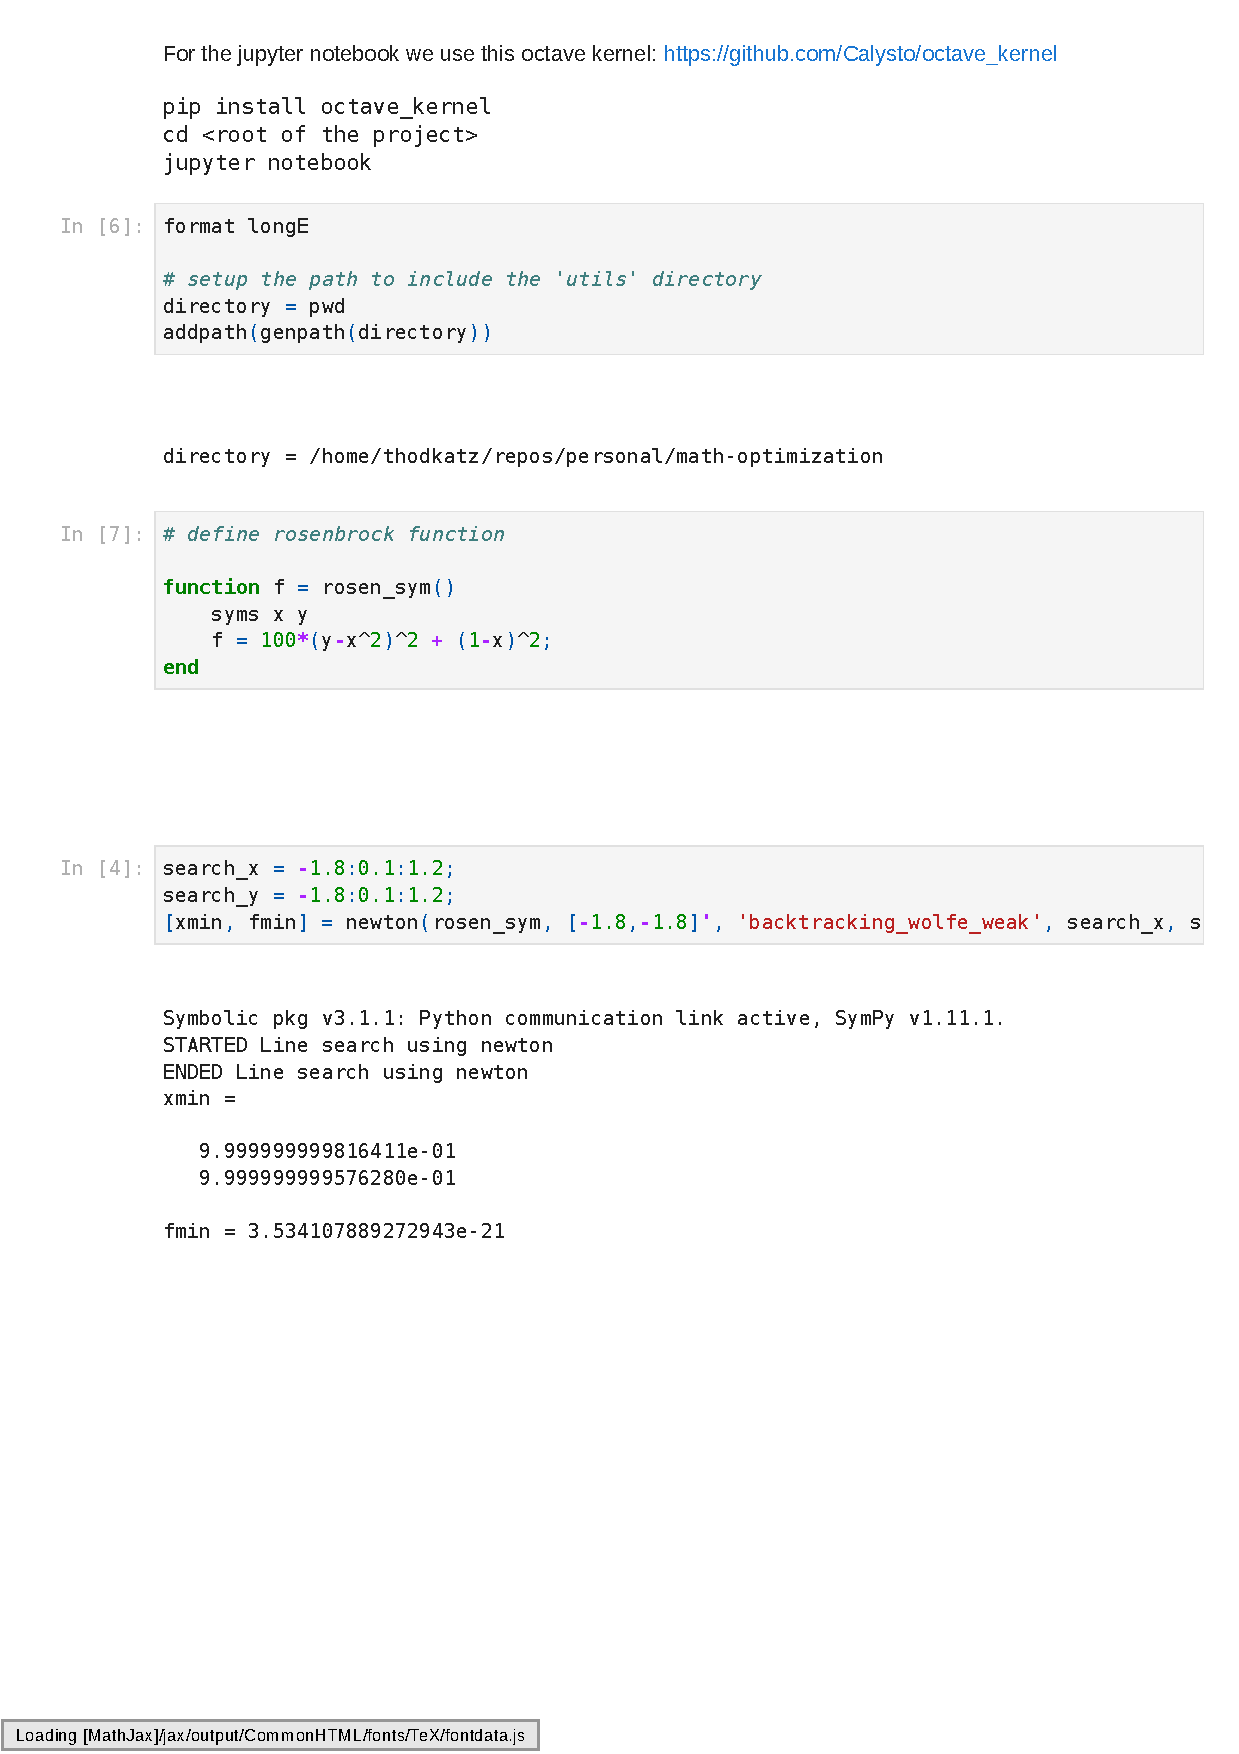
\includepdf[pages=-]{simulation.pdf}


\bibliographystyle{plain}
\bibliography{refs.bib}


\end{document}

